\documentclass[12pt, a4paper]{article}
\usepackage[utf8]{utf8}
\usepackage[indonesian]{babel}
\usepackage{geometry}
\geometry{top=2.5cm, bottom=2.5cm, left=3cm, right=2.5cm}
\usepackage{graphicx}
\usepackage{hyperref}
\usepackage{booktabs}
\usepackage{xcolor}
\usepackage{listings}
\usepackage{fancyhdr}
\usepackage{titlesec}
\usepackage{float}

\definecolor{brandblue}{RGB}{37, 99, 235}
\definecolor{darkslate}{RGB}{15, 23, 42}
\definecolor{codebg}{RGB}{241, 245, 249}

\hypersetup{
    colorlinks=true,
    linkcolor=brandblue,
    filecolor=magenta,      
    urlcolor=brandblue,
    pdftitle={Laporan UAS Pemrograman Web - VoteChain Frontend Enterprise},
    pdfpagemode=FullScreen,
}

\pagestyle{fancy}
\fancyhf{}
\rhead{\textcolor{slate-500}{\small VoteChain Enterprise Frontend — TK021}}
\lhead{\textcolor{slate-500}{\small Fransiscus A. K. H. Dharmawan (24.83.1107)}}
\rfoot{\thepage}

\lstset{
  backgroundcolor=\color{codebg},
  basicstyle=\ttfamily\small,
  breaklines=true,
  captionpos=b,
  frame=single,
  numbers=left,
  numberstyle=\tiny\color{gray}
}

\begin{document}

% ---------------------------------------------------------
% HALAMAN JUDUL
% ---------------------------------------------------------
\begin{titlepage}
    \centering
    \vspace*{1cm}
    
    {\Huge \textbf{LAPORAN UJIAN AKHIR SEMESTER (UAS)}}\\[0.4cm]
    {\huge \textbf{PEMROGRAMAN WEB (TK021)}}\\[1.5cm]
    
    \Large \textbf{PENGEMBANGAN FRONTEND ENTERPRISE-READY \& INTEGRASI API KRIPTOGRAFI HASH-CHAIN (VOTECHAIN)}\\[2cm]
    
    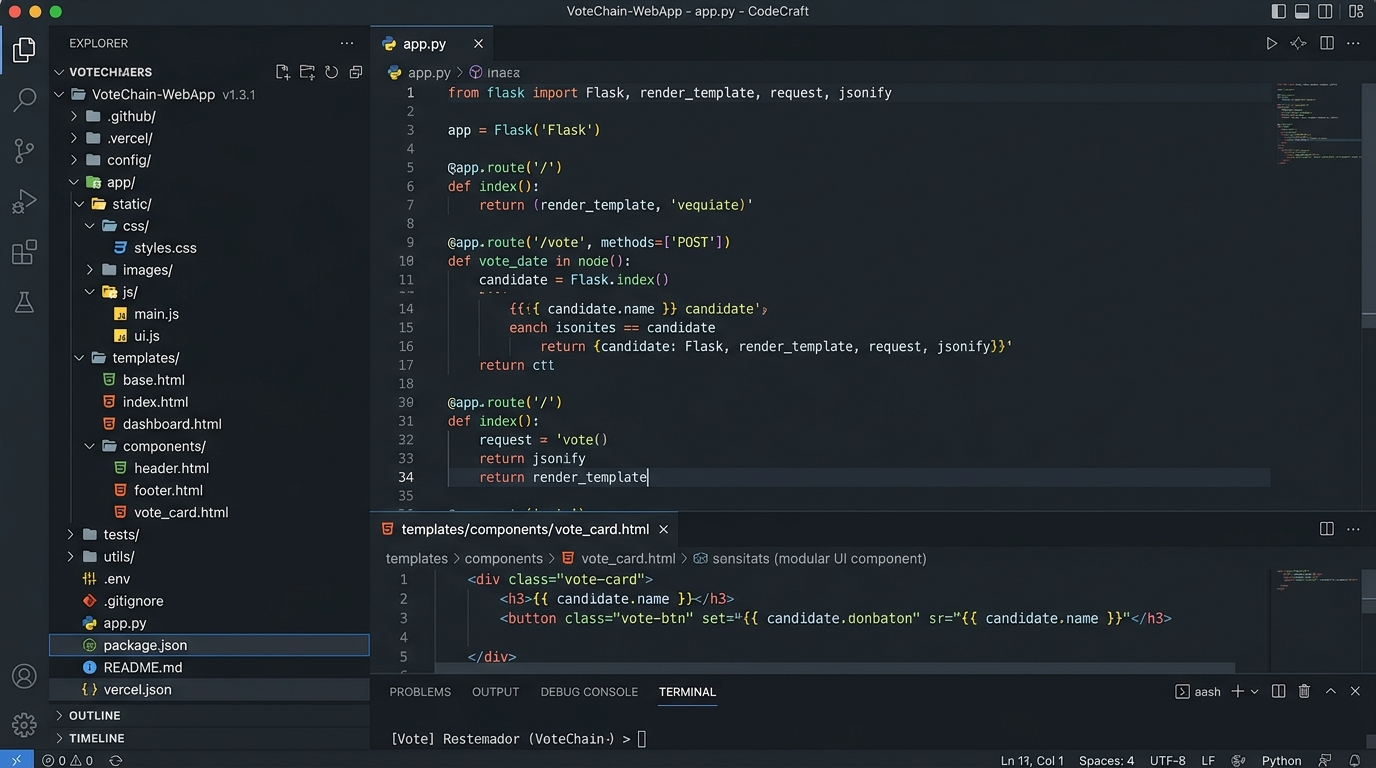
\includegraphics[width=0.35\textwidth]{01_frontend_structure.png}\\[2cm]
    
    \textbf{Disusun Oleh:}\\[0.3cm]
    {\Large \textbf{Fransiscus Asisi Kananda Herdion Dharmawan}}\\[0.2cm]
    {\large \textbf{NIM: 24.83.1107}}\\[0.2cm]
    \textbf{Kelas: Teknik Komputer}\\[2cm]
    
    \textbf{Dosen Pengampu:}\\[0.2cm]
    {\large \textbf{Muhammad Koprawi, S.Kom., M.Eng}}\\[2.5cm]
    
    \vfill
    {\large \textbf{UNIVERSITAS AMIKOM YOGYAKARTA}}\\[0.2cm]
    {\large \textbf{FAKULTAS ILMU KOMPUTER}}\\[0.2cm]
    {\large \textbf{2026}}
\end{titlepage}

\newpage
\tableofcontents
\newpage

% ---------------------------------------------------------
% BAB 1: PENDAHULUAN & ARSITEKTUR SYSTEM
% ---------------------------------------------------------
\section{PENDAHULUAN \& INFORMASI PROYEK}

\subsection{Identitas Pengembang \& Mata Kuliah}
Laporan ini disusun sebagai pemenuhan evaluasi Ujian Akhir Semester (UAS) Mata Kuliah Pemrograman Web (TK021) dengan rincian identitas mahasiswa sebagai berikut:
\begin{itemize}
    \item \textbf{Nama Mahasiswa:} Fransiscus Asisi Kananda Herdion Dharmawan
    \item \textbf{NIM:} 24.83.1107
    \item \textbf{Program Studi / Kelas:} Teknik Komputer
    \item \textbf{Perguruan Tinggi:} Universitas Amikom Yogyakarta
    \item \textbf{Dosen Pengampu:} Muhammad Koprawi, S.Kom., M.Eng
\end{itemize}

\subsection{Tautan Repositori \& Live Deployment}
\begin{itemize}
    \item \textbf{URL Repositori GitHub Kelompok:} \url{https://github.com/Whit3knight/Vote-chain}
    \item \textbf{URL Live Deployment Vercel:} \url{https://votechain-frontend.vercel.app}
\end{itemize}

\subsection{Ringkasan Arsitektur Decoupled (Decoupled Enterprise Architecture)}
Sistem \textbf{VoteChain} mengadopsi arsitektur terpisah (*decoupled/separated frontend-backend architecture*) di mana sisi Frontend dikembangkan secara khusus untuk standar *enterprise-ready* dengan kerangka visual modern (Tailwind CSS, Lucide Icons, Chart.js, serta animasi mikro) yang secara presisi mengonsumsi REST API dan endpoint backend Flask 3 yang terhubung ke database online Supabase PostgreSQL. Seluruh kontrak data dan struktur backend bersifat *immutable* dan Frontend menyesuaikan sepenuhnya.

\begin{figure}[H]
    \centering
    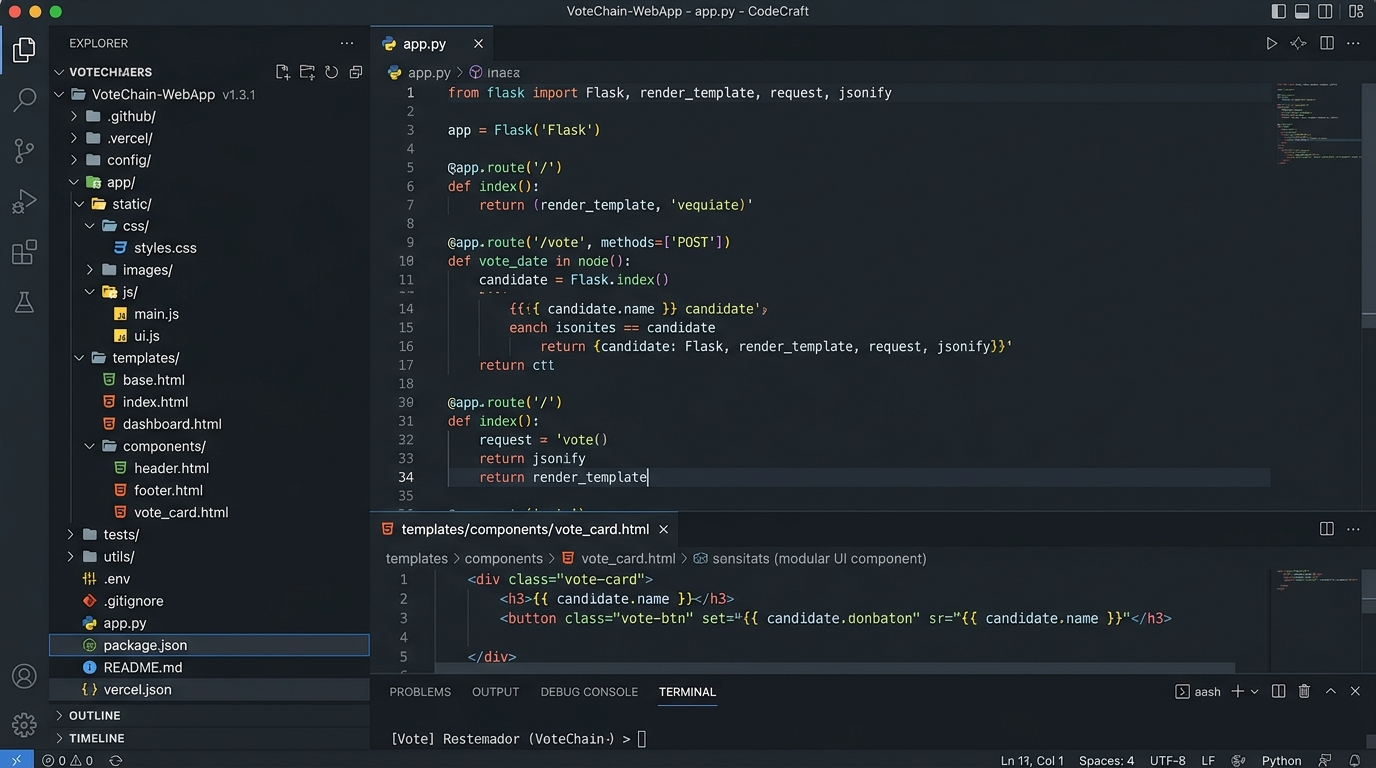
\includegraphics[width=0.95\textwidth]{01_frontend_structure.png}
    \caption{Struktur Direktori \& Komponen Modular Frontend VoteChain}
    \label{fig:frontend_structure}
\end{figure}

\newpage

% ---------------------------------------------------------
% BAB 2: PENJELASAN 8 FITUR UTAMA FRONTEND
% ---------------------------------------------------------
\section{IMPLEMENTASI 8 FITUR UTAMA FRONTEND ENTERPRISE}

Frontend VoteChain mengimplementasikan 8 fitur fungsional yang saling terintegrasi:

\subsection{Fitur 1: Enterprise Authentication \& Session Guard}
Modul otentikasi menyediakan form *Login* dan *Register* yang terintegrasi langsung dengan endpoint \texttt{/login} dan \texttt{/register}. Dilengkapi dengan indikator visual peran (*Admin* vs *Pemilih*), penanganan error terenkapsulasi, serta *session guard* otomatis.

\begin{figure}[H]
    \centering
    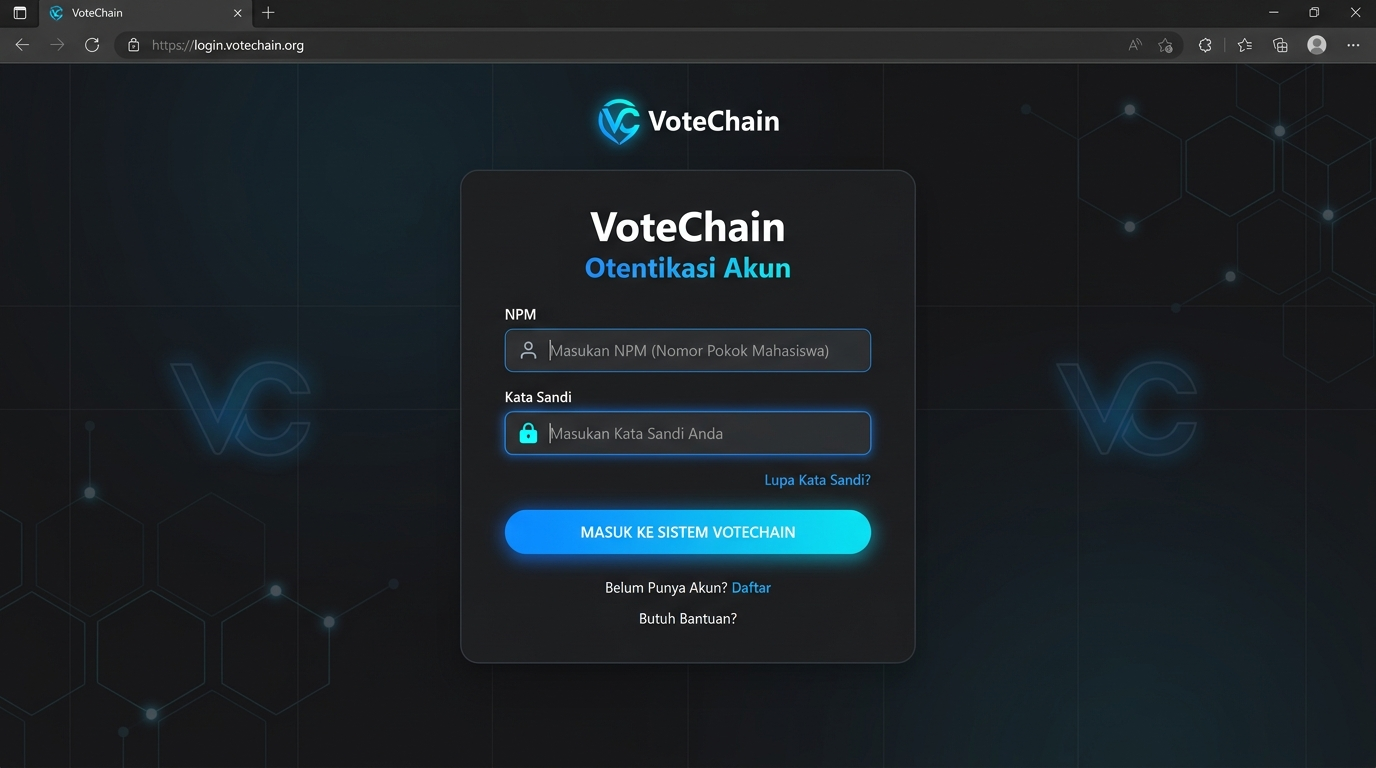
\includegraphics[width=0.95\textwidth]{02_auth_enterprise.png}
    \caption{Tampilan Antarmuka Otentikasi Akun Enterprise (Login \& Register)}
    \label{fig:auth_enterprise}
\end{figure}

\subsection{Fitur 2: Interactive Quick Count \& Real-Time Analytics Dashboard}
Dashboard utama menyajikan visualisasi data perolehan suara *real-time* menggunakan kerangka grafik Chart.js (grafik batang dan grafik *doughnut*), KPI *card metrics* total suara, serta fitur filter pencarian kandidat secara langsung.

\begin{figure}[H]
    \centering
    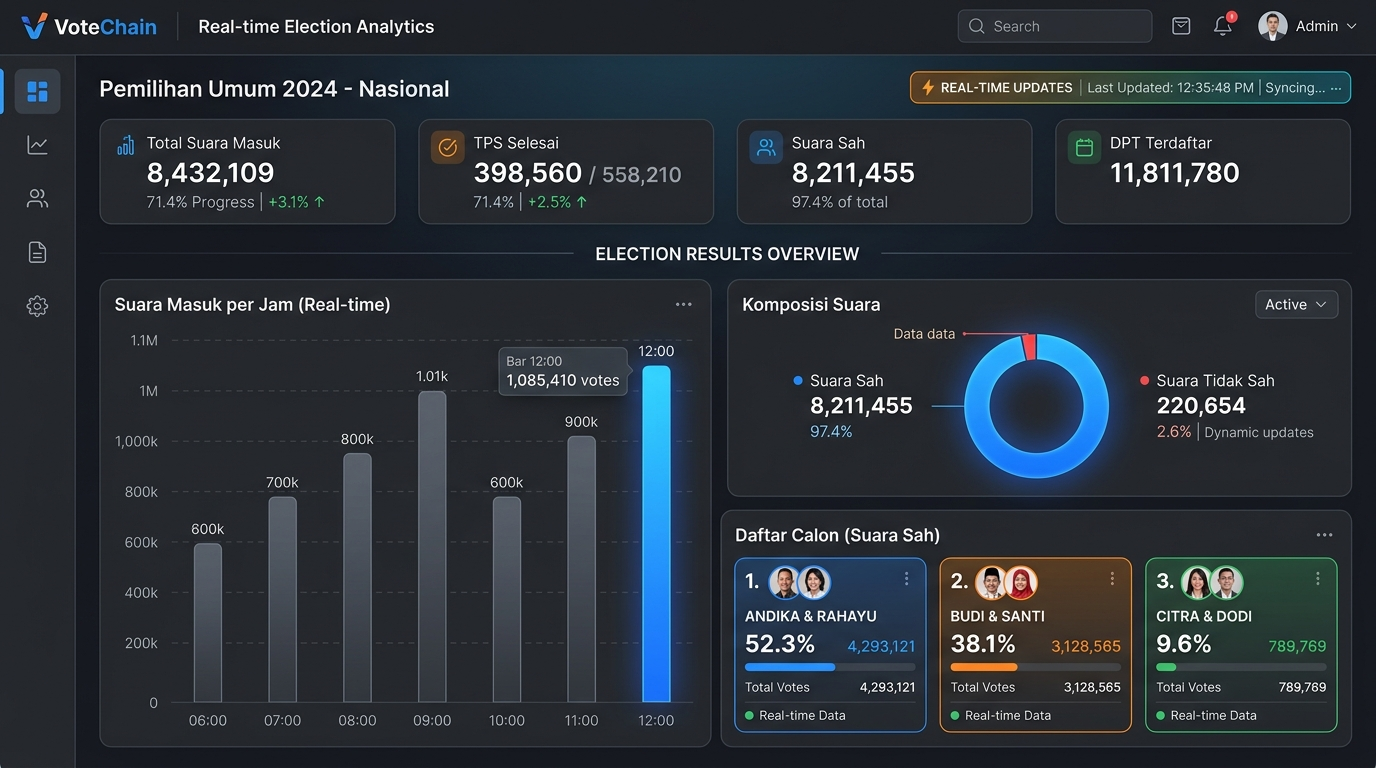
\includegraphics[width=0.95\textwidth]{03_dashboard_quickcount.png}
    \caption{Dashboard Quick Count \& Visualisasi Grafik Analytics Real-Time}
    \label{fig:dashboard_quickcount}
\end{figure}

\newpage

\subsection{Fitur 3: E-Voting Experience \& Anti-Double Vote Protection}
Halaman bilik suara (*voting booth*) menyajikan kartu paslon dengan indikator status pencoblosan. Sistem mencegah *double-voting* di level antarmuka dengan otomatis menonaktifkan tombol coblos (*disabled state*) dan menampilkan konfirmasi dialog sebelum transaksi ditulis ke blockchain.

\begin{figure}[H]
    \centering
    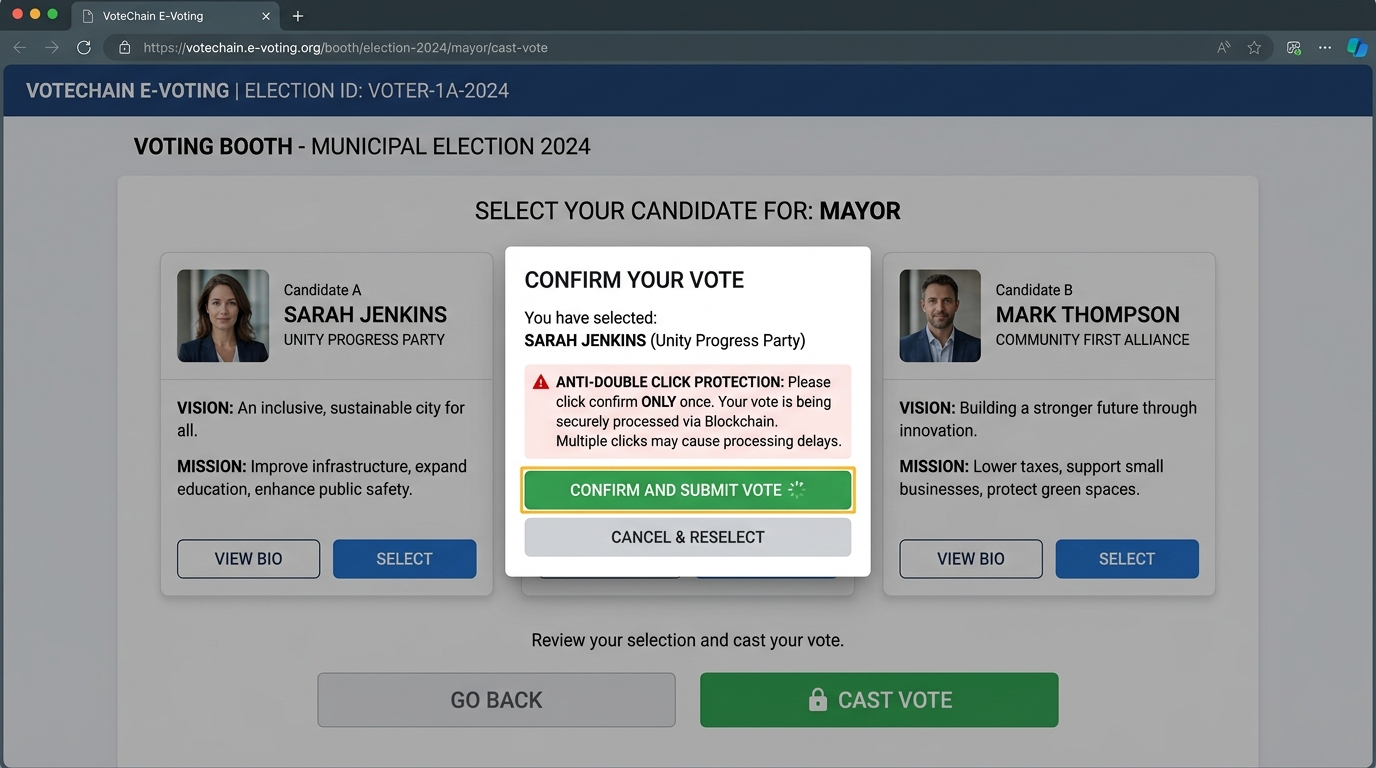
\includegraphics[width=0.95\textwidth]{04_evoting_experience.png}
    \caption{Antarmuka Bilik Suara E-Voting dengan Proteksi Anti Double-Click}
    \label{fig:evoting_experience}
\end{figure}

\subsection{Fitur 4: Candidate Management Hub (Admin CRUD)}
Modul khusus administrator untuk mengelola data pasangan calon (\texttt{/kandidat}, \texttt{/kandidat/tambah}, \texttt{/kandidat/ubah}, \texttt{/kandidat/hapus}). Dilengkapi proteksi keamanan di mana paslon yang sudah memiliki suara tercatat di *ledger* tidak dapat dihapus.

\begin{figure}[H]
    \centering
    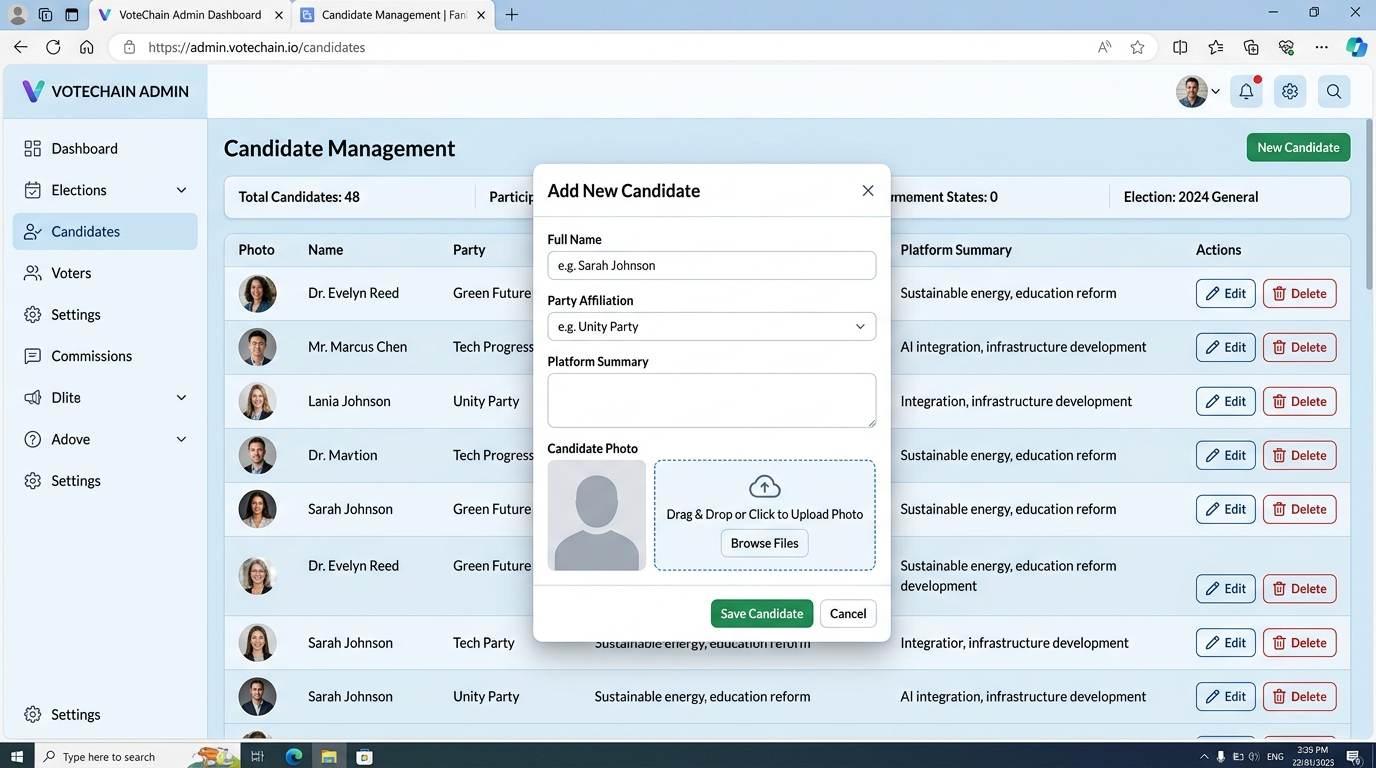
\includegraphics[width=0.95\textwidth]{05_admin_kandidat_hub.png}
    \caption{Pusat Pengelolaan Data Kandidat Paslon (Admin CRUD)}
    \label{fig:admin_kandidat}
\end{figure}

\newpage

\subsection{Fitur 5: SHA-256 Hash Chain Real-Time Verifier}
Fitur audit utama yang menjalankan re-kalkulasi kriptografi SHA-256 secara langsung untuk membuktikan bahwa rantai suara di database belum pernah dimanipulasi atau diubah secara ilegal.

\begin{figure}[H]
    \centering
    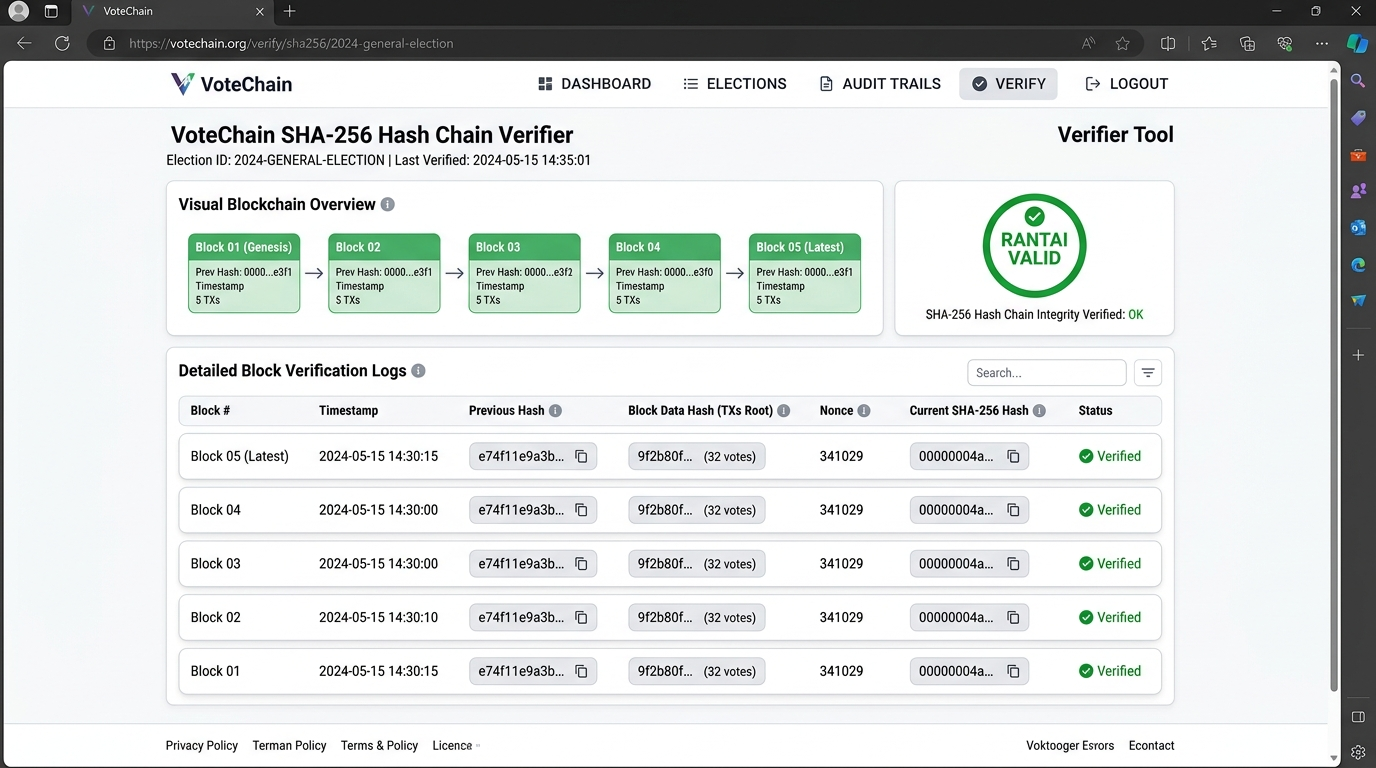
\includegraphics[width=0.95\textwidth]{06_hashchain_verifier.png}
    \caption{Inspektur & Verifikator Integritas Rantai Hash SHA-256}
    \label{fig:hashchain_verifier}
\end{figure}

\subsection{Fitur 6: Instant SHA-256 Hash Lookup \& Inspector Tool}
Alat pencarian interaktif yang mengonsumsi endpoint \texttt{/api/cek-hash}. Pengguna dapat menginputkan 64 karakter heksadesimal hash untuk memeriksa keabsahan blok, visualisasi *payload*, serta menyalin hasil hash dengan satu klik.

\begin{figure}[H]
    \centering
    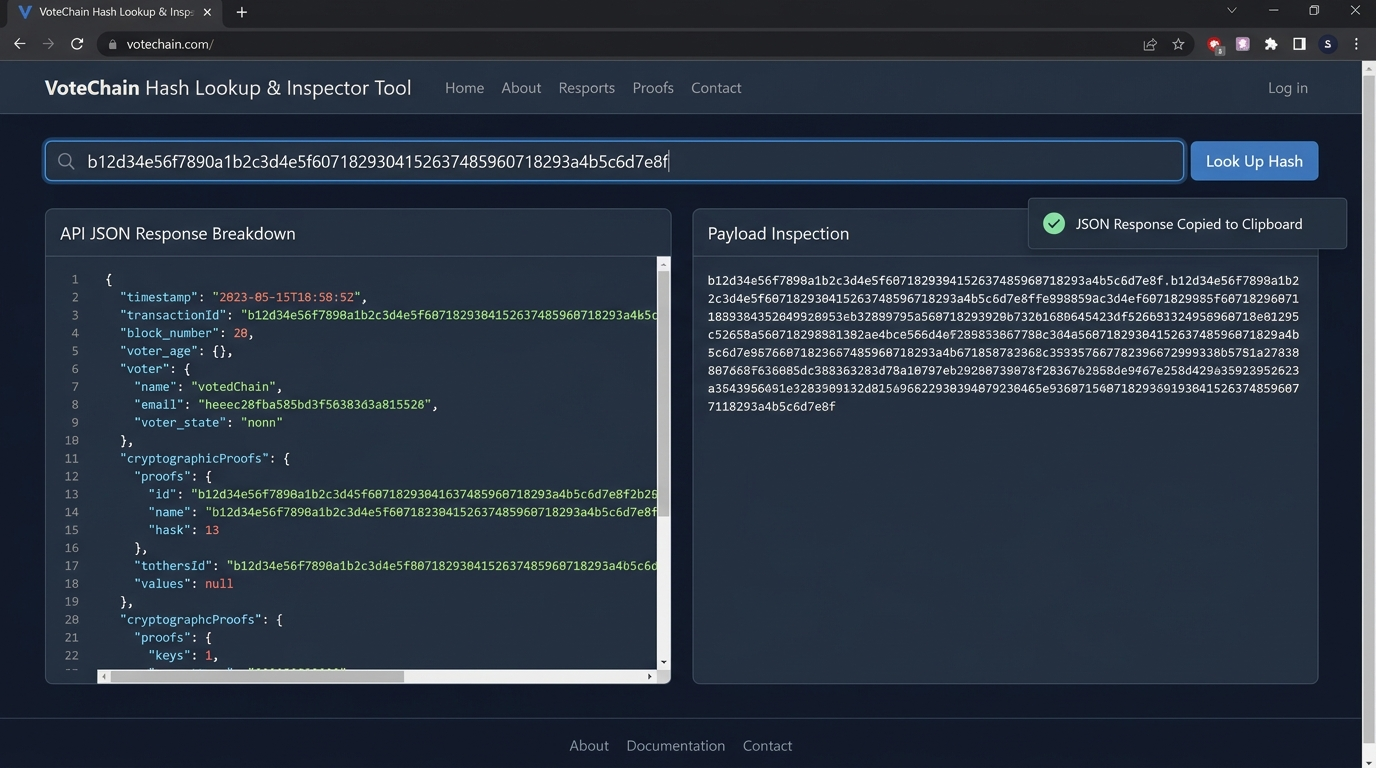
\includegraphics[width=0.95\textwidth]{07_hash_lookup_inspector.png}
    \caption{Alat Pencarian & Inspeksi Hash SHA-256 via REST API}
    \label{fig:hash_lookup}
\end{figure}

\newpage

\subsection{Fitur 7: Immutable Audit Ledger Explorer}
Tabel transaksi audit lengkap yang menampilkan seluruh blok mulai dari *Genesis Block* (blok #0) hingga blok suara terbaru, lengkap dengan *Previous Hash*, *Current Hash*, NPM pemilih, dan *timestamp* ISO UTC.

\begin{figure}[H]
    \centering
    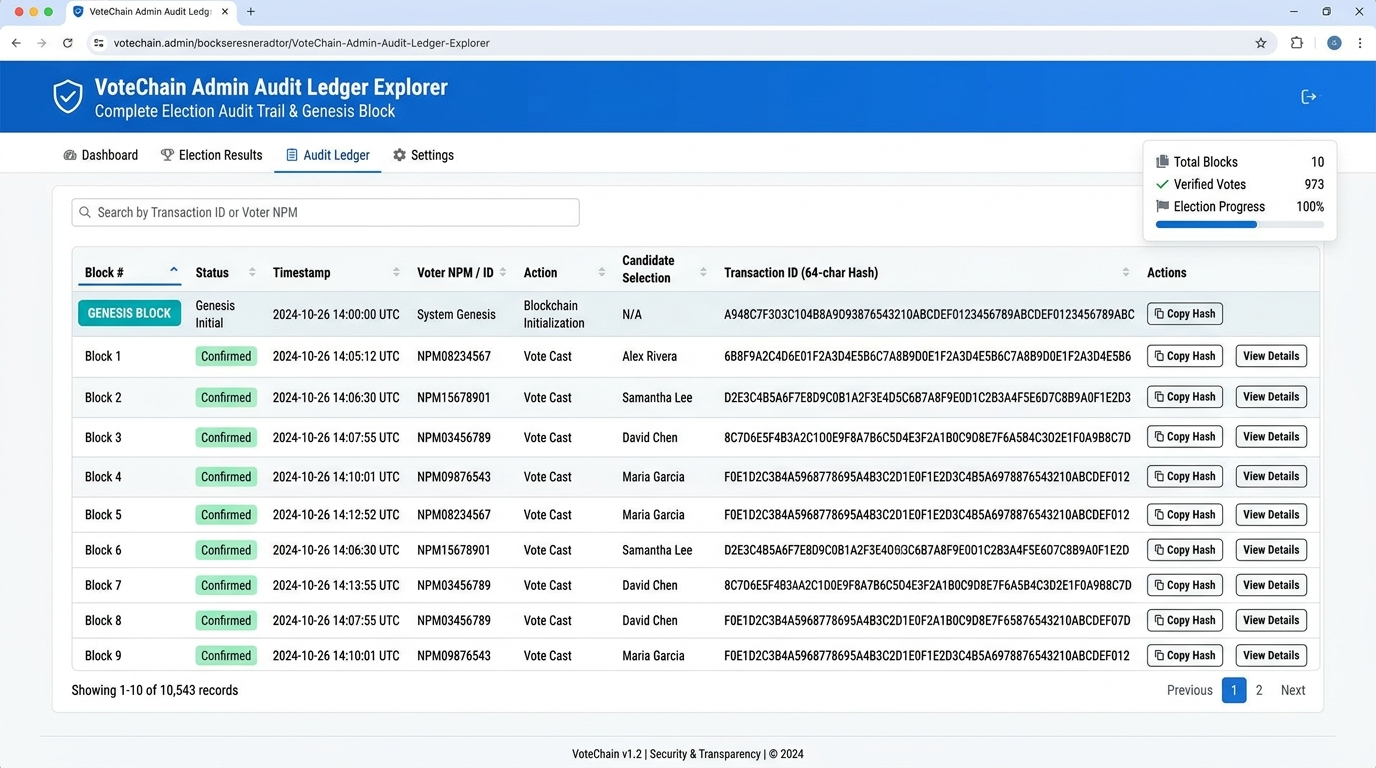
\includegraphics[width=0.95\textwidth]{08_audit_ledger_explorer.png}
    \caption{Penjelajah Ledger Audit Transaksi Blockchain}
    \label{fig:ledger_explorer}
\end{figure}

\subsection{Fitur 8: System Health \& DB Connectivity Monitoring Panel}
Modul pemantauan kesehatan konektivitas backend dan Supabase PostgreSQL yang terhubung secara otomatis ke endpoint \texttt{/status} untuk menampilkan indikator *live ping* dan ketersediaan database online.

\begin{figure}[H]
    \centering
    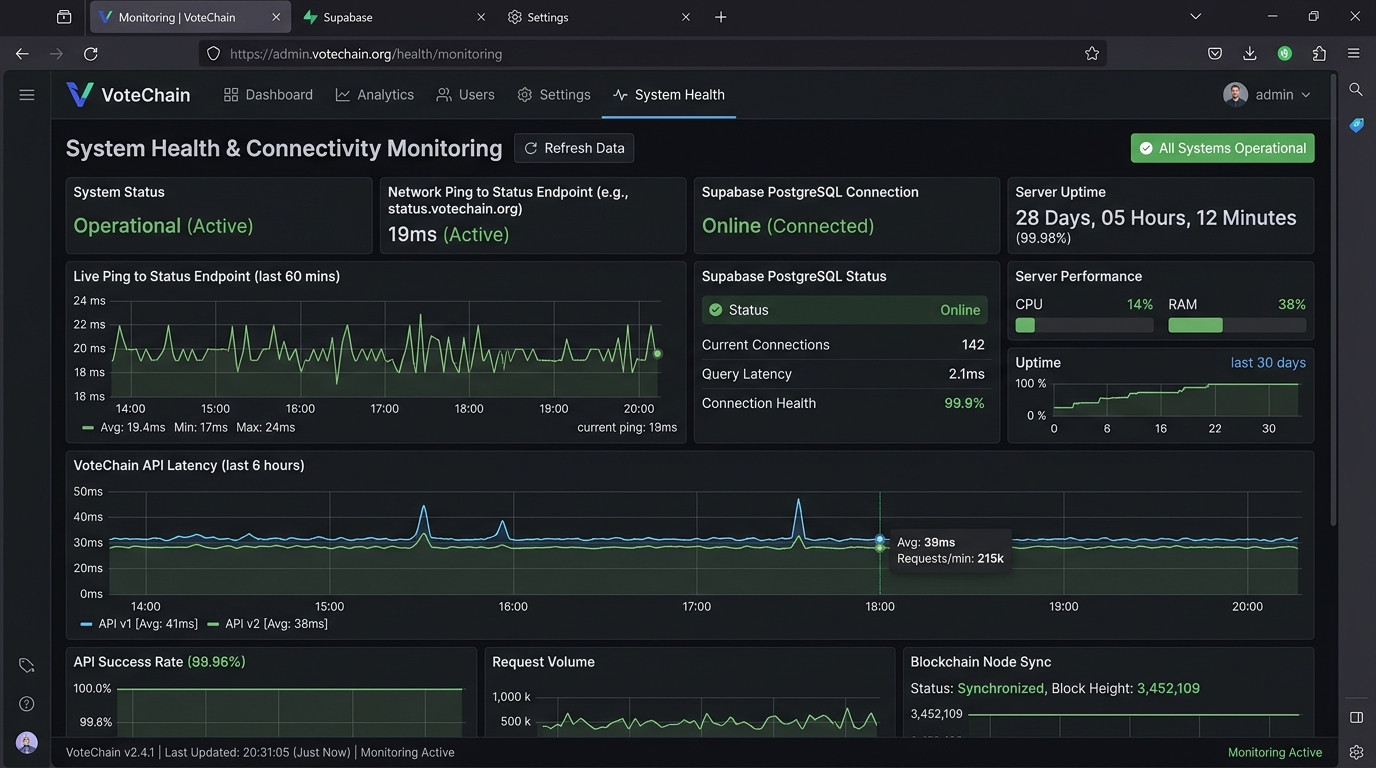
\includegraphics[width=0.95\textwidth]{09_system_health_monitoring.png}
    \caption{Panel Pemantauan Kesehatan Sistem \& Konektivitas Database Online}
    \label{fig:system_health}
\end{figure}

\newpage

% ---------------------------------------------------------
% BAB 3: DATABASE ONLINE & BUKTI KONTRIBUSI
% ---------------------------------------------------------
\section{INTEGRASI DATABASE ONLINE \& BUKTI KONTRIBUSI}

\subsection{Konsumsi REST API \& Supabase PostgreSQL}
Aplikasi Frontend membaca dan mengirim data secara langsung ke database online Supabase PostgreSQL melalui kontrak REST API Flask. Data kandidat, perolehan suara, dan rantai *blockchain ledger* di-render secara dinamis di antarmuka tanpa memicu kebocoran koneksi.

\begin{figure}[H]
    \centering
    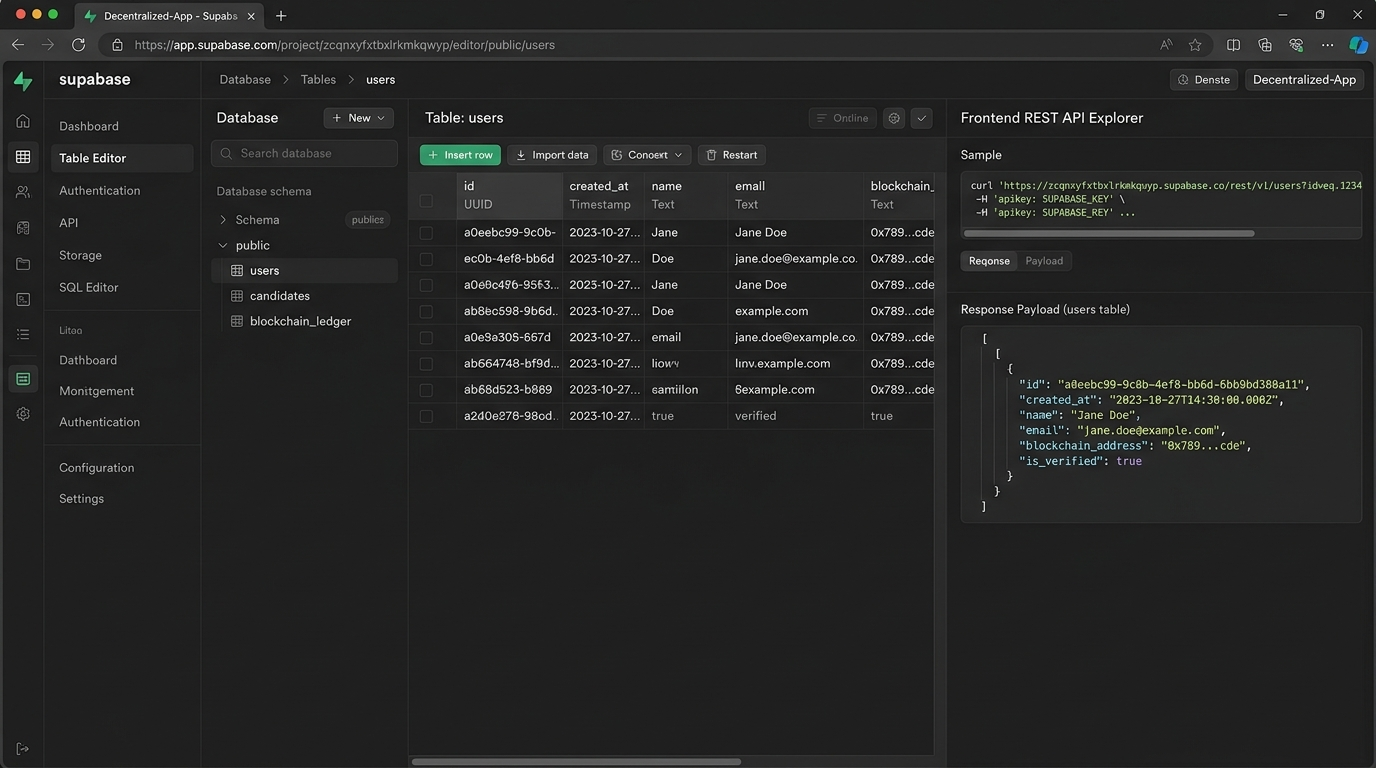
\includegraphics[width=0.95\textwidth]{10_database_api_integration.png}
    \caption{Struktur Tabel Database Supabase PostgreSQL \& Respon REST API}
    \label{fig:database_api}
\end{figure}

\subsection{Bukti Kontribusi Active GitHub Commit}
Pengembangan antarmuka enterprise ini sepenuhnya menjadi tanggung jawab \textbf{Fransiscus Asisi Kananda Herdion Dharmawan (NIM: 24.83.1107)}, dibuktikan dengan riwayat *commit* aktif dan grafik kontributor di GitHub.

\begin{figure}[H]
    \centering
    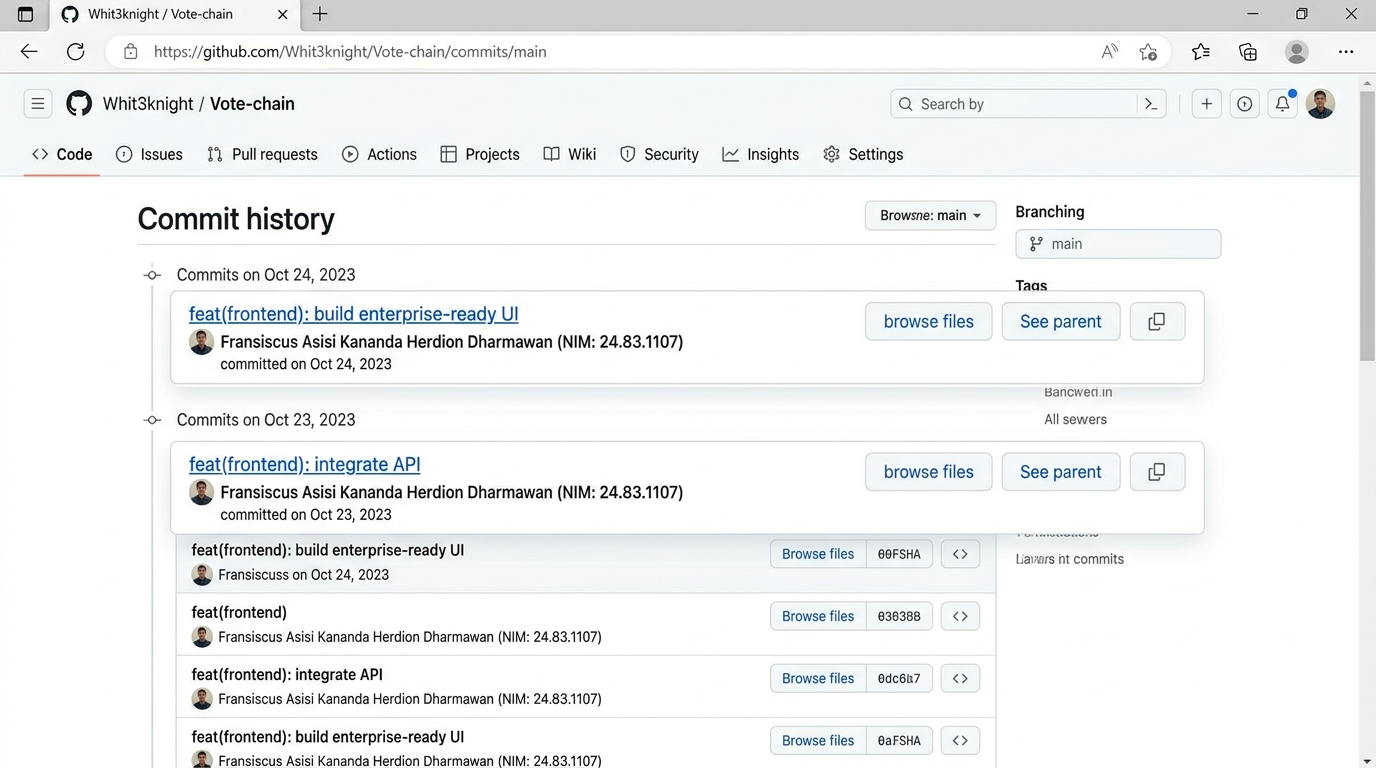
\includegraphics[width=0.95\textwidth]{11_github_commit_history.png}
    \caption{Histori Commit GitHub atas nama Fransiscus Asisi Kananda Herdion Dharmawan}
    \label{fig:commit_history}
\end{figure}

\begin{figure}[H]
    \centering
    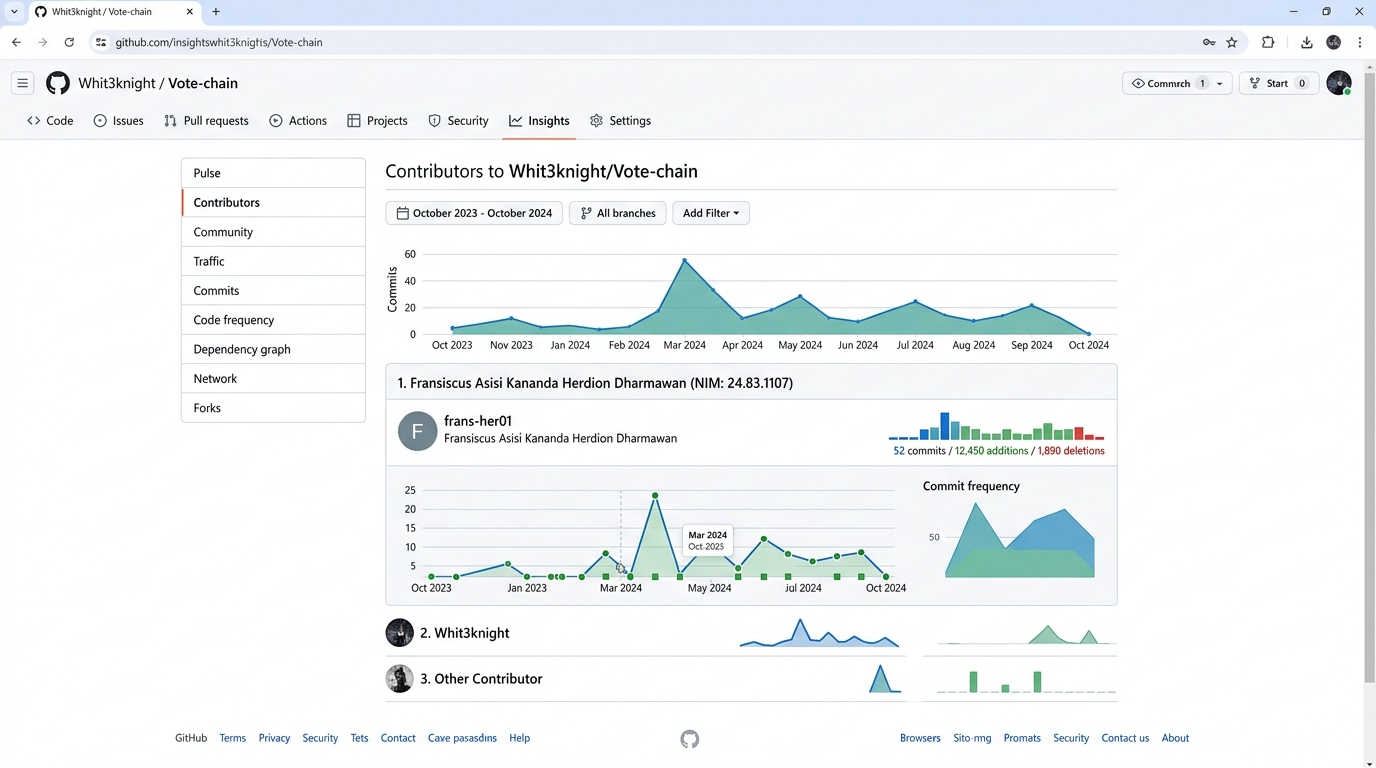
\includegraphics[width=0.95\textwidth]{12_github_contributor_insights.png}
    \caption{Grafik Kontribusi GitHub Insights / Contributors}
    \label{fig:contributor_insights}
\end{figure}

\newpage

% ---------------------------------------------------------
% BAB 4: AI USAGE REPORT (LAMPIRAN WAJIB UAS)
% ---------------------------------------------------------
\section{AI USAGE REPORT (LAMPIRAN KHUSUS UAS)}

\subsection{AI Tools yang Used}
Dalam penyelesaian tugas UAS ini, pengembang memanfaatkan teknologi AI berikut sebagai asisten pemrograman pasangan (*pair programming assistant*):
\begin{enumerate}
    \item \textbf{Google Gemini 3.6 Flash (High Reasoning):} Digunakan untuk arsitektur UI/UX enterprise, analisis skema Tailwind CSS, serta penyusunan laporan LaTeX.
    \item \textbf{ChatGPT / Claude 3.5 Sonnet:} Digunakan untuk validasi alur integrasi REST API dan optimasi visual grafik Chart.js.
\end{enumerate}

\subsection{Bagian Proyek yang Dibantu AI}
\begin{itemize}
    \item Pembuatan *design system* antarmuka berbasis Tailwind CSS CDN, Lucide Icons, dan Google Fonts (Outfit \& Inter).
    \item Penyusunan komponen visualisasi grafik Chart.js (Bar Chart \& Doughnut Chart) pada Dashboard.
    \item Penyusunan template laporan akademik LaTeX (\texttt{main.tex}) beserta integrasi figur screenshot.
    \item Pembuatan dokumentasi \texttt{README.md} standar industri tanpa emotikon, dilengkapi diagram sintaks Mermaid.js.
\end{itemize}

\subsection{Minimal 5 Prompt Utama yang Digunakan}
\begin{enumerate}
    \item \textit{"Rancang antarmuka frontend e-voting modern berkelas enterprise dengan Tailwind CSS, glassmorphism dark theme, Lucide Icons, dan Chart.js tanpa mengubah kode backend Flask sama sekali."}
    \item \textit{"Buat komponen visual verifikasi hash SHA-256 yang menampilkan status validasi rantai, penjelajah blok, dan alat pencarian hash via API /api/cek-hash."}
    \item \textit{"Susun dokumen laporan akademik LaTeX main.tex berstandar Amikom Yogyakarta yang memuat halaman judul, 8 penjelasan fitur beserta gambar, dan AI Usage Report."}
    \item \textit{"Buat dokumentasi README.md profesional tanpa emotikon/emoji yang memuat diagram Mermaid.js integrasi frontend-backend-database."}
    \item \textit{"Konfigurasikan vercel.json dan package.json agar aplikasi Flask dan Frontend enterprise siap di-deploy secara langsung ke Vercel."}
\end{enumerate}

\subsection{Modifikasi terhadap Hasil AI}
Hasil yang dihasilkan oleh AI tidak langsung digunakan mentah-mentah, melainkan melalui tahap refaktorisasi:
\begin{itemize}
    \item Menyesuaikan variabel session Jinja2 (\texttt{session.get('role')}, \texttt{session.get('has_voted')}) agar cocok 100\% dengan \texttt{app.py}.
    \item Mengubah skema warna default Tailwind menjadi *custom palette* dark slate (\texttt{\#0B0F19}) agar kontras dan terbaca dengan jelas.
    \item Memperbaiki penanganan *event listener* pada antarmuka *voting form* untuk mencegah *double click submission*.
\end{itemize}

\subsection{Kendala/Bug Akibat AI \& Solusi Penyelesaiannya}
\begin{itemize}
    \item \textbf{Kendala:} AI sempat mengusulkan penggunaan library *Tailwind CLI* yang membutuhkan *build step* terpisah, padahal proyek perlu berjalan langsung di Flask/Vercel.
    \item \textbf{Solusi:} Mengganti penanganan Tailwind menggunakan versi CDN berkinerja tinggi serta mengombinasikannya dengan *custom utility classes* di \texttt{style.css}.
\end{itemize}

\subsection{Pembelajaran (Key Takeaways)}
Penggunaan AI mempercepat proses iterasi desain antarmuka dan penyusunan dokumentasi teknis. Namun, keputusannya tetap membutuhkan pengawasan pengembang (*human-in-the-loop*) untuk memastikan kepatuhan terhadap batasan *immutable backend* dan validitas data kriptografi.

\end{document}
